In this section, we describe our approach to generating 3D
exemplar-based templates on-the-fly. It is based on 3D CAD model
rendering (Sect.~\ref{sec:rendering}) followed by feature extraction
and applying a whitening procedure. Based on the original whitening
formulation (Sect.~\ref{sec:who}), we propose three novel extensions that
enable the application of whitening to the on-the-fly setting.
%
First, we adapt the whitening to the specific case of rendered
images (Sect.~\ref{sec:nzwho}). Second, we show how to speed up the
whitening by two orders of magnitudes for high-resolution templates
(Sect.~\ref{sec:fastwhiten}). And third, we improve the runtime of our
3D exemplar template detectors also at test time, by performing
convolutions in the frequency domain (Sect.~\ref{sec:fft}).


\subsection{Rendering}
\label{sec:rendering}

We used an off-the-shelf rendering engine that can create a realistic rendering and
a depth map. The CAD models we used contain color, texture and material information such as
transparency and reflectance to make the rendering as realistic
as possible to simulate the natural image statistics. An rendering example that we used in our experiments is
in Fig. \ref{fig:rendering}. Along with a rendering, we extracted a depth map which can later 
be used for reconstruction.

To handle intraclass variability, we used various CAD models (sedan, truck, racing car, hatchback etc) to cover intraclass variability and made renderings of these CAD models for various viewpoints. The
CAD models were cached so that when we fine-tune 2D-3D matching, we can render the model instantaneously.
Our renderer can continuously vary yaw, pitch, roll and the focal length as well so that the final fine tuning stage produces accurate the continuous viewpoint, a focal length and a bounding box.

\begin{figure}[t]
  \begin{center}
     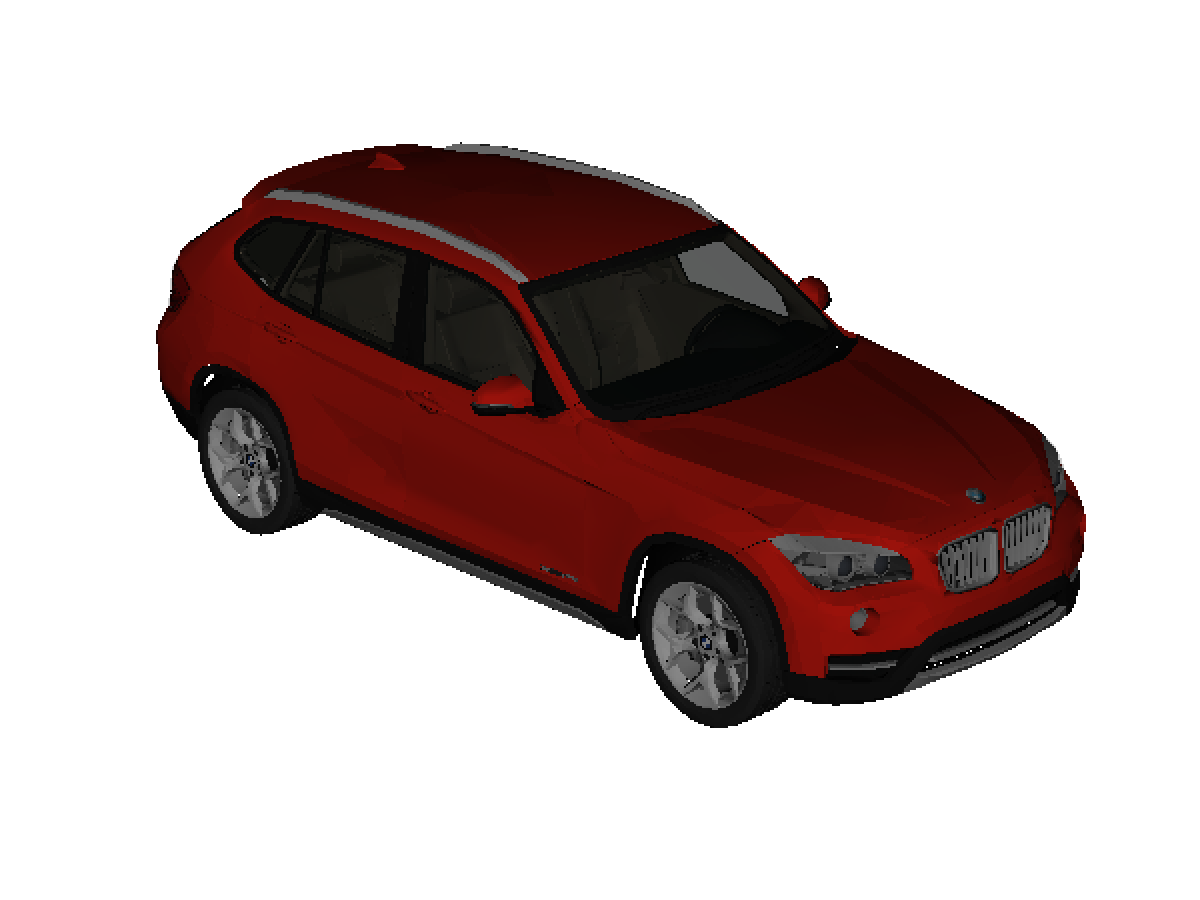
\includegraphics[width=0.4\linewidth]{rendering}
     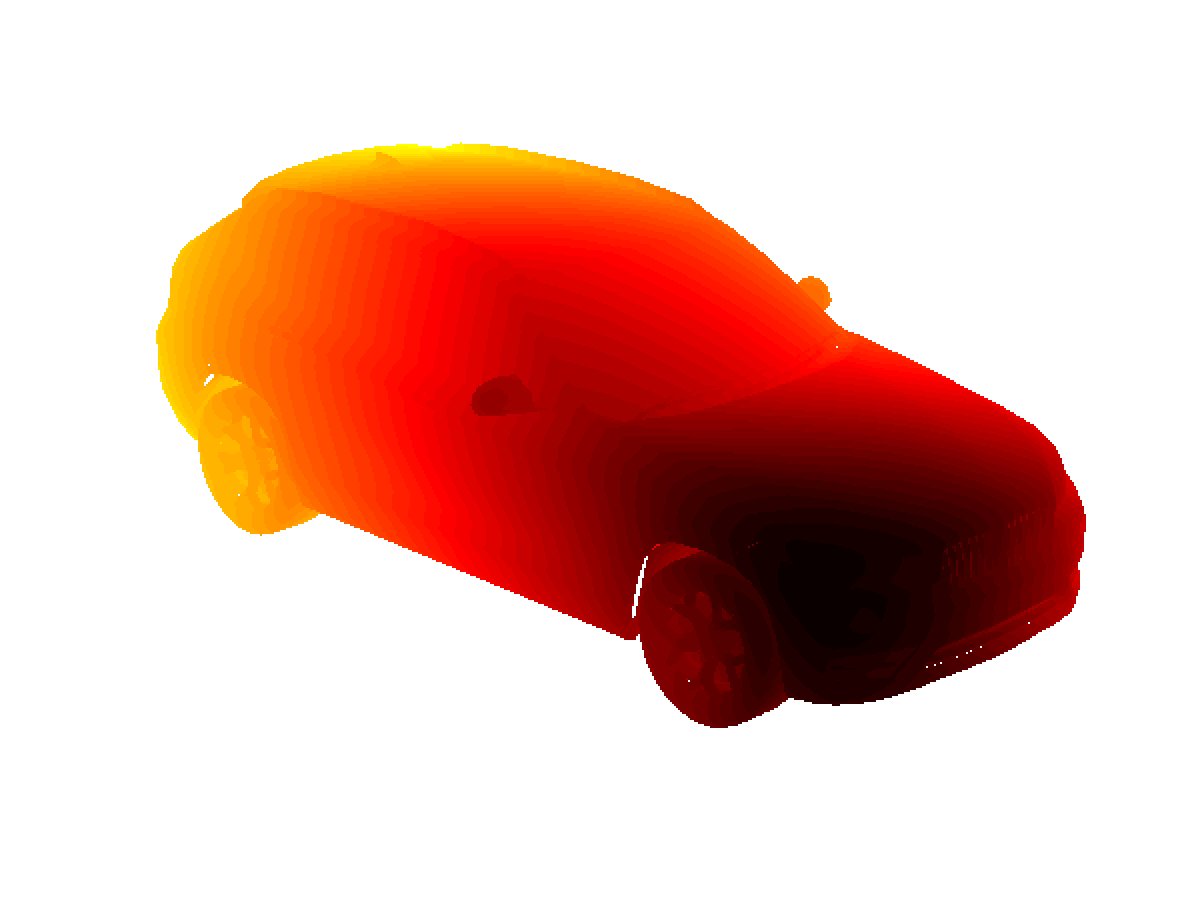
\includegraphics[width=0.4\linewidth]{depth}
  \end{center}
  \caption{An example rendering and depth image from renderer.}
  \label{fig:rendering}
\end{figure}


\subsection{Whitened Histograms of Orientations (WHO)}
\label{sec:who}
Our technique for rendering and generating exemplar template detectors on-the-fly
is drawing from recent work. Hariharan \etal. introduced Whitened Histograms of Orientations (WHO)
\cite{Hariharan12}, which uses feature statistics from natural images to whiten HOG
templates, making them more discriminative. Whitening is a common signal
processing operation for decorrelating a set of random variables
\cite{Martinsson05, Belouchrani00}. More formally, suppose that we have a
$k$-dimensional random variable $X \in \mathcal{R}^k$ with $Cov(X)=\Sigma$. By
whitening the signal,

\begin{equation}
\tilde{X}=\Sigma^{-\frac{1}{2}}(X - E[X]) \label{eq:whitening},
\end{equation}

we remove 2nd order correlation between all features. Since collecting covariance
matrix for every template shape is expensive, \cite{Hariharan12} proposed an easy
way to synthesize
covariance $\Sigma$ from autocovariance $\Gamma$ and we followed their
method to generate $\Sigma$.


% More formally, suppose that we have a
% $k$-dimensional random variable $X \in \mathcal{R}^k$ with $Cov(X)=\Sigma$. By
% whitening the signal,
% \begin{equation}
% \tilde{X}=\Sigma^{-\frac{1}{2}}(X - E[X]) \label{eq:whitening},
% \end{equation}

% Since collecting covariance matrix for every template shape
%  is expensive, \cite{Hariharan12} proposed easy way to synthesize
% covariance $\Sigma$ from autocovariance $\Gamma$ and we followed their
% method to generate $\Sigma$.

% The whitening and LDA have the same
% formulation when we make a decision boundary $w = \Sigma^{-1}(\mu_+ - \mu_0)$
% where $\mu_+$ is the features from a class (LDA) or a signal to whiten
% (whitening), $\mu_0$ is the negative class center (LDA) or the signal mean
% (whitening) and $\Sigma$ is the covariance matrix of classes (LDA) or
% the correlation within signal (whitening).

% In \cite{Hariharan12}, the authors compute the mean and covariance matrix by assuming Wide-Sense Stationarity (WSS) of HOG features
% generated from natural images. That is, they assume the mean of a HOG cell is
% independent of its place in the image, and the autocovariance of cells depends
% only on their relative location.

% In one dimension, let $x(u)$ be the feature at location $u$. Then WSS states
% that $\mathbb{E}\left[x(u)\right] = \mu$ for all $u$, and
% \begin{equation}
% \textrm{cov}_x(u,v) = \textrm{cov}_x(0, v-u) = \Gamma(v-u),
% \end{equation} where $\Gamma$ is the autocovariance. For simplicity, we describe the 1D case but this can be easily extended to 2D spatial autocovariance.
% 
% Therefore, assuming WSS allows the covariance matrix of templates \emph{of any
% size} to be synthesized from the autocovariance matrix using a simple lookup.

% However, the 
% We propose Non-Zero Whitened Histograms of Orientations (NZ-WHO), that are both
% more discriminative than WHO, and can be generated several orders of magnitude
% faster (in 70ms compared to several seconds for WHO). This speed up means we
% can generate templates on the fly, allowing our approach to evaluate arbitrary
% viewpoint hypotheses.

% Our method requires generating a covariance matrix of non-zero cells 

\subsection{Whitening Synthesized Templates and Non-Zero WHO}
\label{sec:nzwho}
Our first innovation is `Non-Zero' whitening. When synthesizing detection
templates from rendered images, a common problem is how to handle the
background. If the model is rendered over a natural image background, gradients
in the background will be incorporated into the discriminative template,
potentially causing false-positives if background elements exist in the query
image.

Alternatively, if the background is left textureless (see
Fig.~\ref{fig:rendering}), whitening the resulting HOG template
will produce undesirable background artifacts. These are created when centering
the template (by subtracting the mean $\mu$), where strong negative weights are
introduced in the textureless region (as seen in Fig.~\ref{fig:whocomparison}).
This could result in positive matches being suppressed due to spurious
background gradients.

NZ-WHO removes these artifacts so that the background has no effect on the
template response. Let a vectorized HOG features of a rendering image $x\in
\mathcal{R}^{nd}$ be $x=T_f(I_r)$ where $n$ is the number HOG cells and $d$ be
the dimension of HOG feature. We create a new vector $x'$ which contains only
the non-zero elements of $x$. To be specific, let $I_d\in \mathcal{R}^{d\times
    d}$ be the identity matrix, $n'$ be the number of non-zero HOG cells, and a
matrix $S\in \mathcal{R}^{n'd \times nd}$ be the masking matrix that selects
non-zero HOG cell. For instance, a template has  $n=3, n'=2$, and only the
second HOG cell has $0$ norm, then

\begin{align}
S = \left[ \begin{array}{ccc}
        I_d & \mathbf{0} & \mathbf{0}\\
        \mathbf{0} & \mathbf{0} & I_d
        \end{array} \right]
\end{align}

Then, we can define $x' = S x, \mu' = S\mu, \Sigma' = S \Sigma S^T$.
After solving the resulting system (which is now smaller than
in the WHO approach) we find

\begin{equation}
w'=\Sigma'^{-1}(x' - \mu') \label{eq:nz-who},
\end{equation}

which we restore zero cells and reshape the vector into the final NZ-WHO
template that has the same dimension as the original HOG template.

% Notice that $\Sigma$ is not square-rooted in Eq.~\ref{eq:nz-who}, whereas it is
% in the definition of whitening (Eq.~\ref{eq:whitening}). This is because the
% whitened template will only be used in the context of detection, which involves
% the inner product with the whitened HOG features of the query image $y$:
% \begin{equation}
% (y-\mu)^{T}\Sigma^{-\frac{1}{2}}\Sigma^{-\frac{1}{2}}(x-\mu)\\
% = (y-\mu)^{T} w.
% \end{equation}
% We can therefore capture the whitening of the query image features in $w$.

% We use the GPU to parallelize the lookup of the correct autocovariance cells during covariance matrix syntheses, which is \scream{x} times faster than using the CPU (Figure \ref{fig:covariancetime}).

%\scream{chris:We propose Non-Zero Whitened Histograms of Orientations (NZ-WHO), an improvement over WHO which is both more discriminative than WHO and can be computed many orders of magnitude faster than WHO (70ms as opposed to to several seconds for WHO). This speedup allows us to generate NZ-WHO templates on the fly, allowing us to quickly evaluate arbitrary viewpoint hypotheses.}
%\scream{add comments about the fig:whocomparison}

\begin{figure}[t]
  \begin{center}
%   \fbox{\rule{0pt}{2in} \rule{0.9\linewidth}{0pt}}
    % include whitening all centered cells
    % 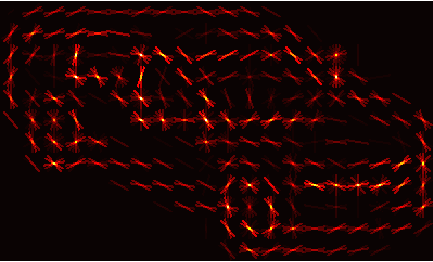
\includegraphics[width=0.32\linewidth]{whiten_all_crop}
    \setlength\tabcolsep{3pt}
    \begin{tabular}{ccc}
      HOG & WHO & NZ-WHO \\
%     \begin{turn}{90}$w_+$\end{turn} &
    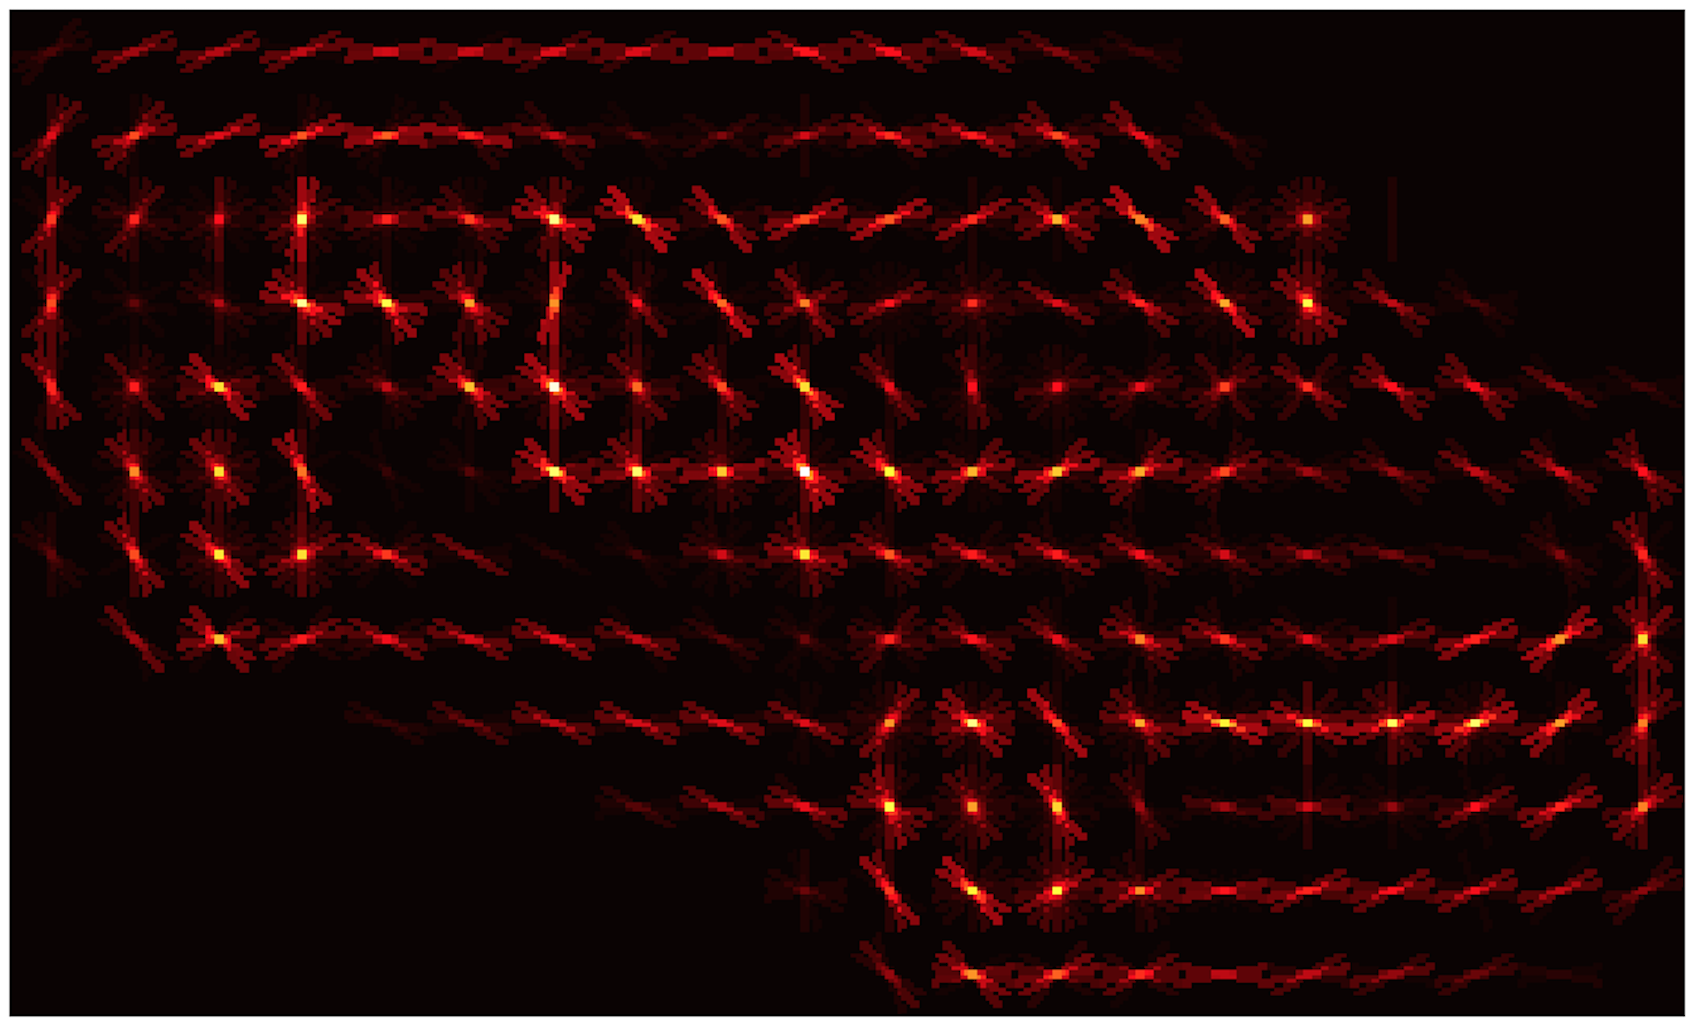
\includegraphics[width=0.28\linewidth]{hog_crop} &
    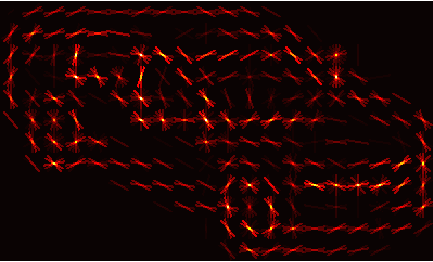
\includegraphics[width=0.28\linewidth]{whiten_all_crop} &
    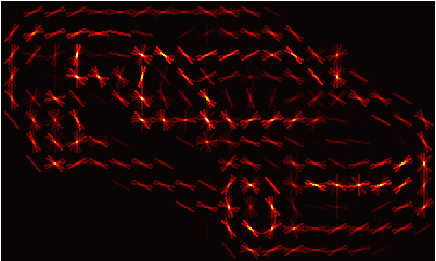
\includegraphics[width=0.28\linewidth]{whiten_non_zero_crop} \\
    % include whitening all centered cells
     % 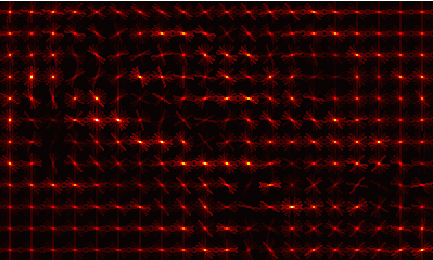
\includegraphics[width=0.282\linewidth]{whiten_all_neg_crop} 
%     \begin{turn}{90}$-w_-$\end{turn} &
     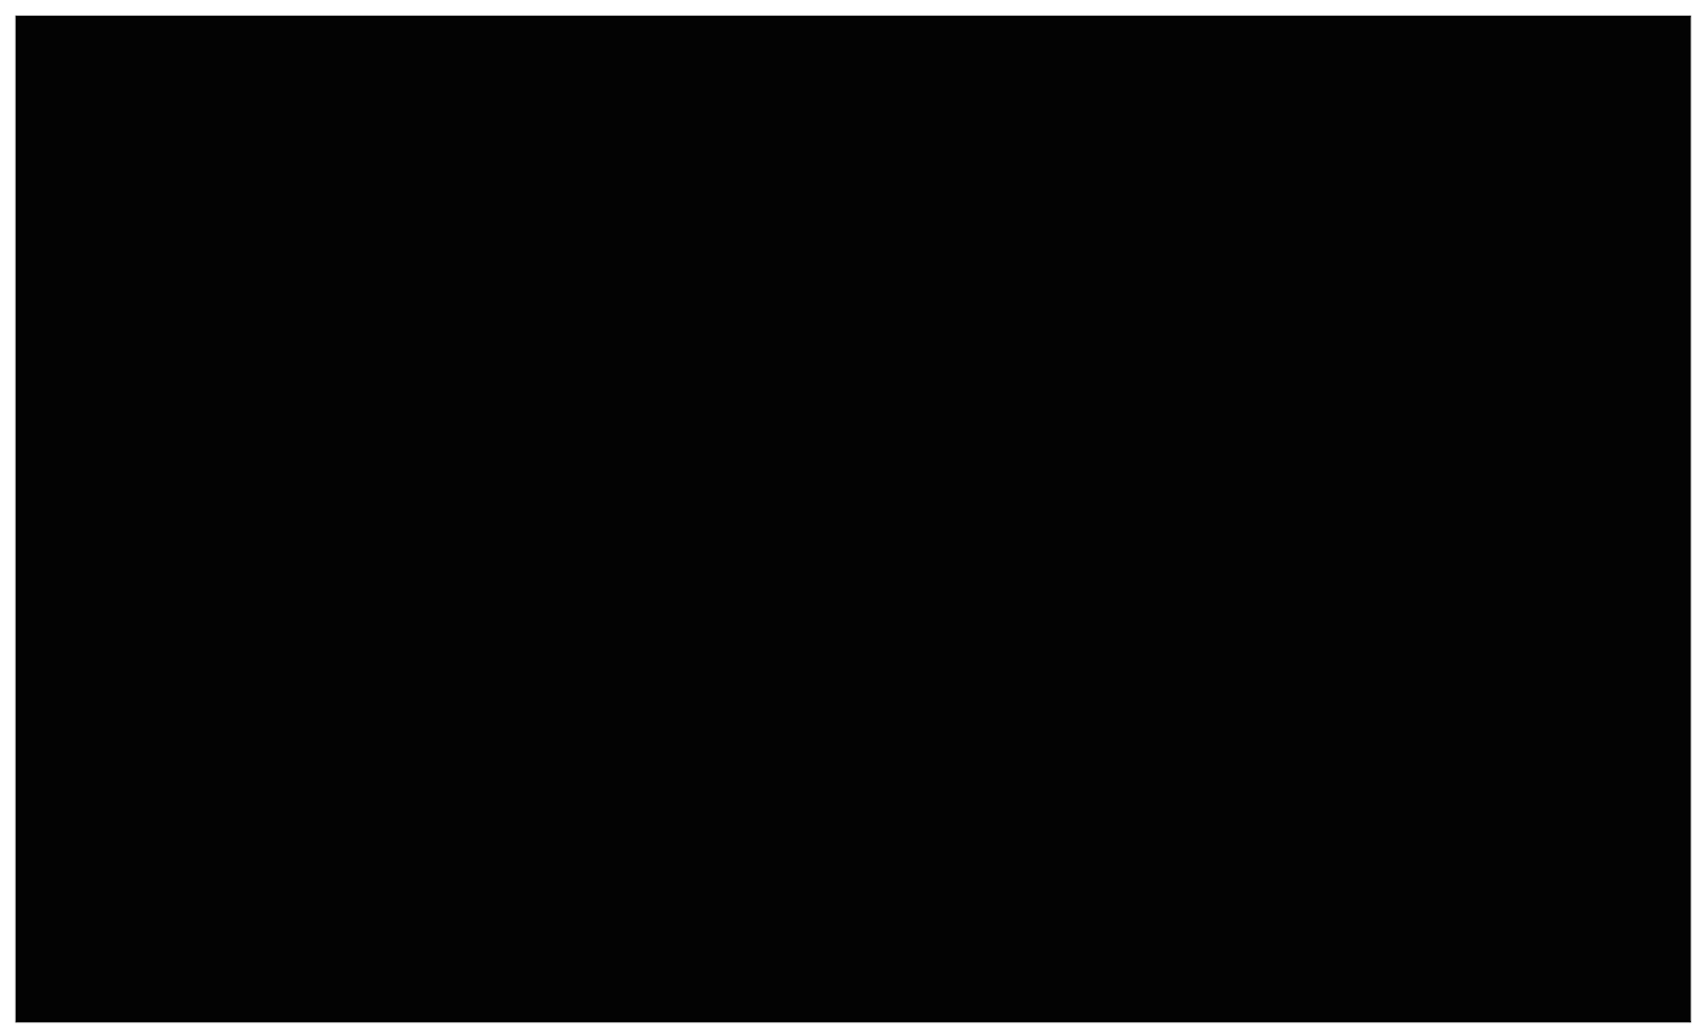
\includegraphics[width=0.28\linewidth]{hog_neg_crop} &
     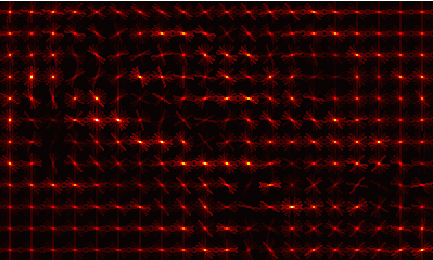
\includegraphics[width=0.28\linewidth]{whiten_all_neg_crop}  &
     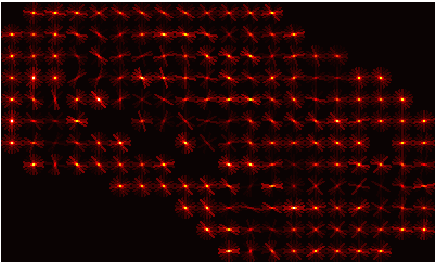
\includegraphics[width=0.28\linewidth]{whiten_non_zero_neg} \\
    % include whitening all centered cells
 %    \begin{turn}{90}ihog\cite{vondrick2013}\end{turn} &
    % \cite{vondrick2013}& 
     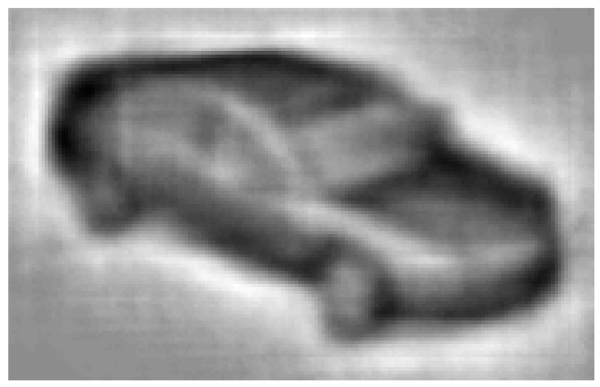
\includegraphics[width=0.28\linewidth]{ihog_hog200_crop.png} &
     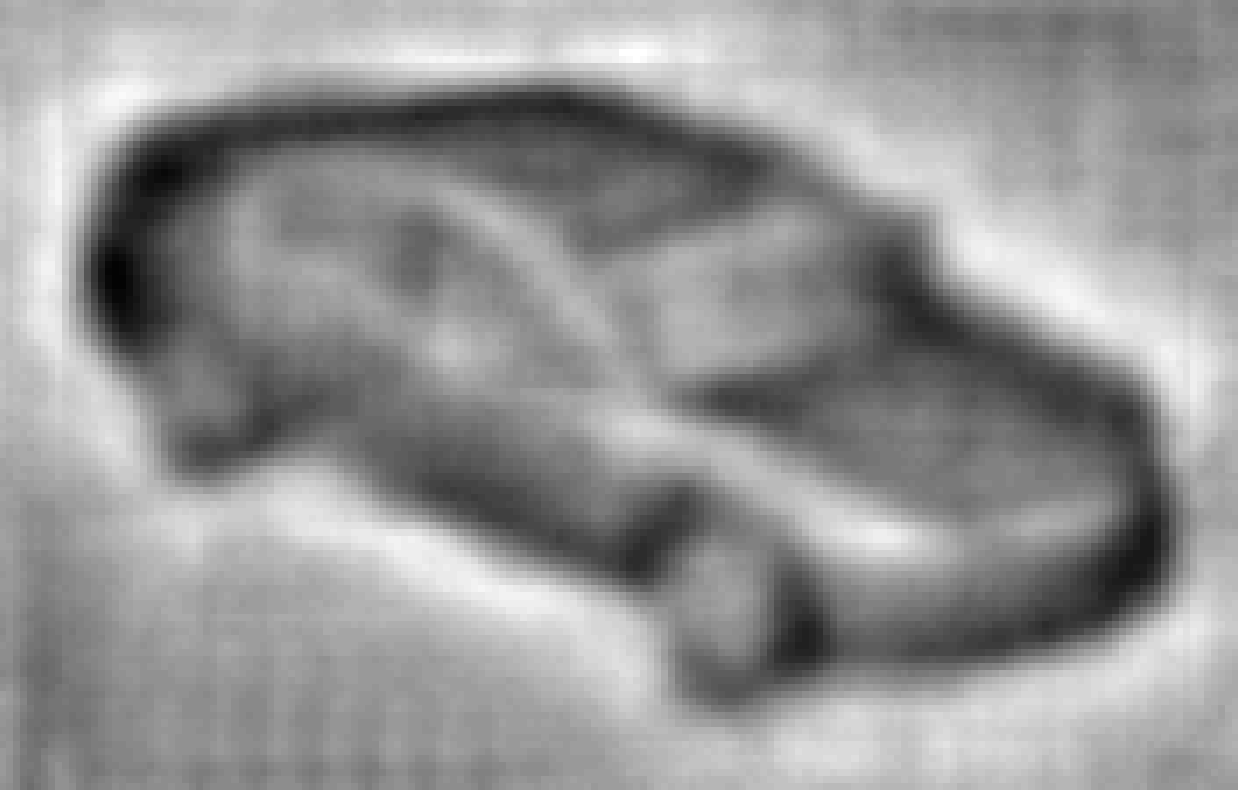
\includegraphics[width=0.28\linewidth]{ihog_whiten_all200_crop.png} &
     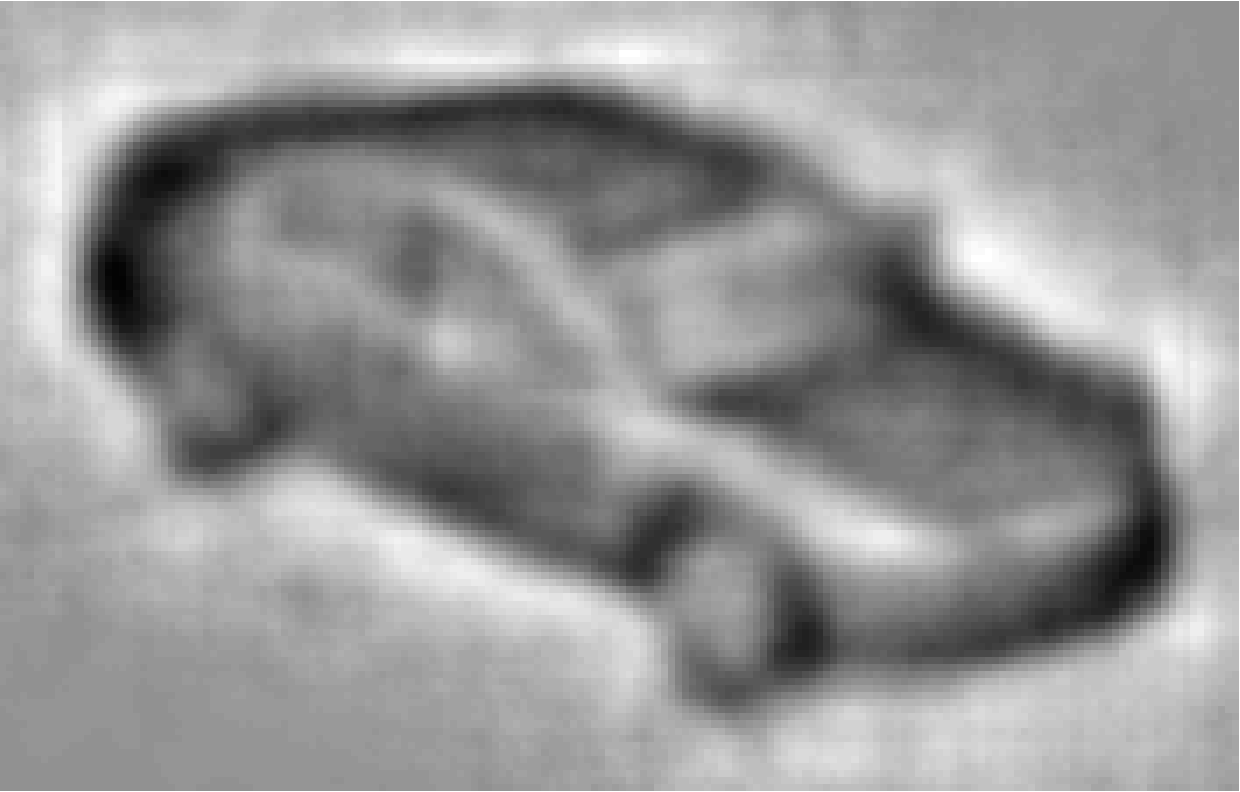
\includegraphics[width=0.28\linewidth]{ihog_whiten_non_zero200_crop.png} \\
 \end{tabular}
  \end{center}
  \caption{Comparison of HOG, WHO and NZ-WHO. Visualization of positive weights (first row),  visualization of negative weights (second row), HOGgles \cite{vondrick2013} (third row). Note that for WHO, whitening all cell result in strong negative edges on the empty region}
  \label{fig:whocomparison}
\end{figure}


\subsection{Fast Whitening using Conjugate Gradient}
\label{sec:fastwhiten}
Our second innovation lies in enhancing the computational efficiency
of the whitening procedure, making it applicable to an on-the-fly
rendering setting.

It originates from the insight that an iterative
Conjugate Gradient method can be used to whiten a HOG template, which
is much faster than the original procedure proposed
in~\cite{Hariharan12} based on decomposition.

Whitening the non-zero
feature vector $x'$ means a solving the system of linear equations, $\Sigma' w' = (x' -
\mu')$. In
\cite{Hariharan12}, the authors make use of the fact that covariance matrices
are symmetric and positive semidefinite to solve the system via the Cholesky
decomposition with Gaussian Elimination, which requires $O(n^3)$ time.

The Conjugate Gradient method is an iterative algorithm for solving symmetric
positive definite systems which runs in $O(n^2\kappa)$ time, where $\kappa$ is
the condition number of the matrix. \cite{Shewchuk94}.
%
This makes Conjugate Gradient faster than decomposition for matrices with small condition
numbers relative to their size.

The covariance matrix for HOG templates is typically
ill-conditioned\cite{Hariharan12}, but we
can add a regularization constant to the diagonal to reduce its condition
number to the point where the conjugate gradient method will converge quickly.
We use a constant of $0.15$, which reduces the condition number from $10^{20}$
to $50$, much smaller than the dimension of the matrix (7000).

As a result, a GPU implementation of conjugate gradient converges in 80
ms when using 250 HOG cells, two orders of magnitude faster than the using
Cholesky factorization with Gaussian Elimination.


We report the real time analysis of whitening using decomposition and
conjugate gradient methods in Fig.~\ref{fig:whotime}. (a) compares the
absolute runtime of the different methods while (b) gives the obtained
speedup. We see that % We compare the speed of each of template generation methods in
% Fig.~\cite{fig:covariancetime_crop} Using naive Cholesky decomposition,
WHO template takes several seconds for realistic template sizes of
several hundred cells, while using the iterative Conjugate Gradient
method, it only takes 80ms. If we use NZ-WHO, we can gain extra speed
up since we only whitens non-zero cells.

In addition, since the iterative Conjugate Gradient method directly
tries to reduce the residual (the norm of $y-Ax$ for $Ax = y$), it is
more numerically stable than Cholesky decomposition with Gaussian
Elimination. We vary the number of cells in a template and show that
the residual of NZ-WHO is smaller than WHO Fig.~\ref{fig:whoresidual}.
% Also, the residual from the Conjugate Gradient method (the norm of $y-Ax$ for $Ax = y$) is smaller than 
% that of Cholesky decomposition. 

\begin{figure}[t]
  \begin{center}
  \begin{tabular}{cc}
     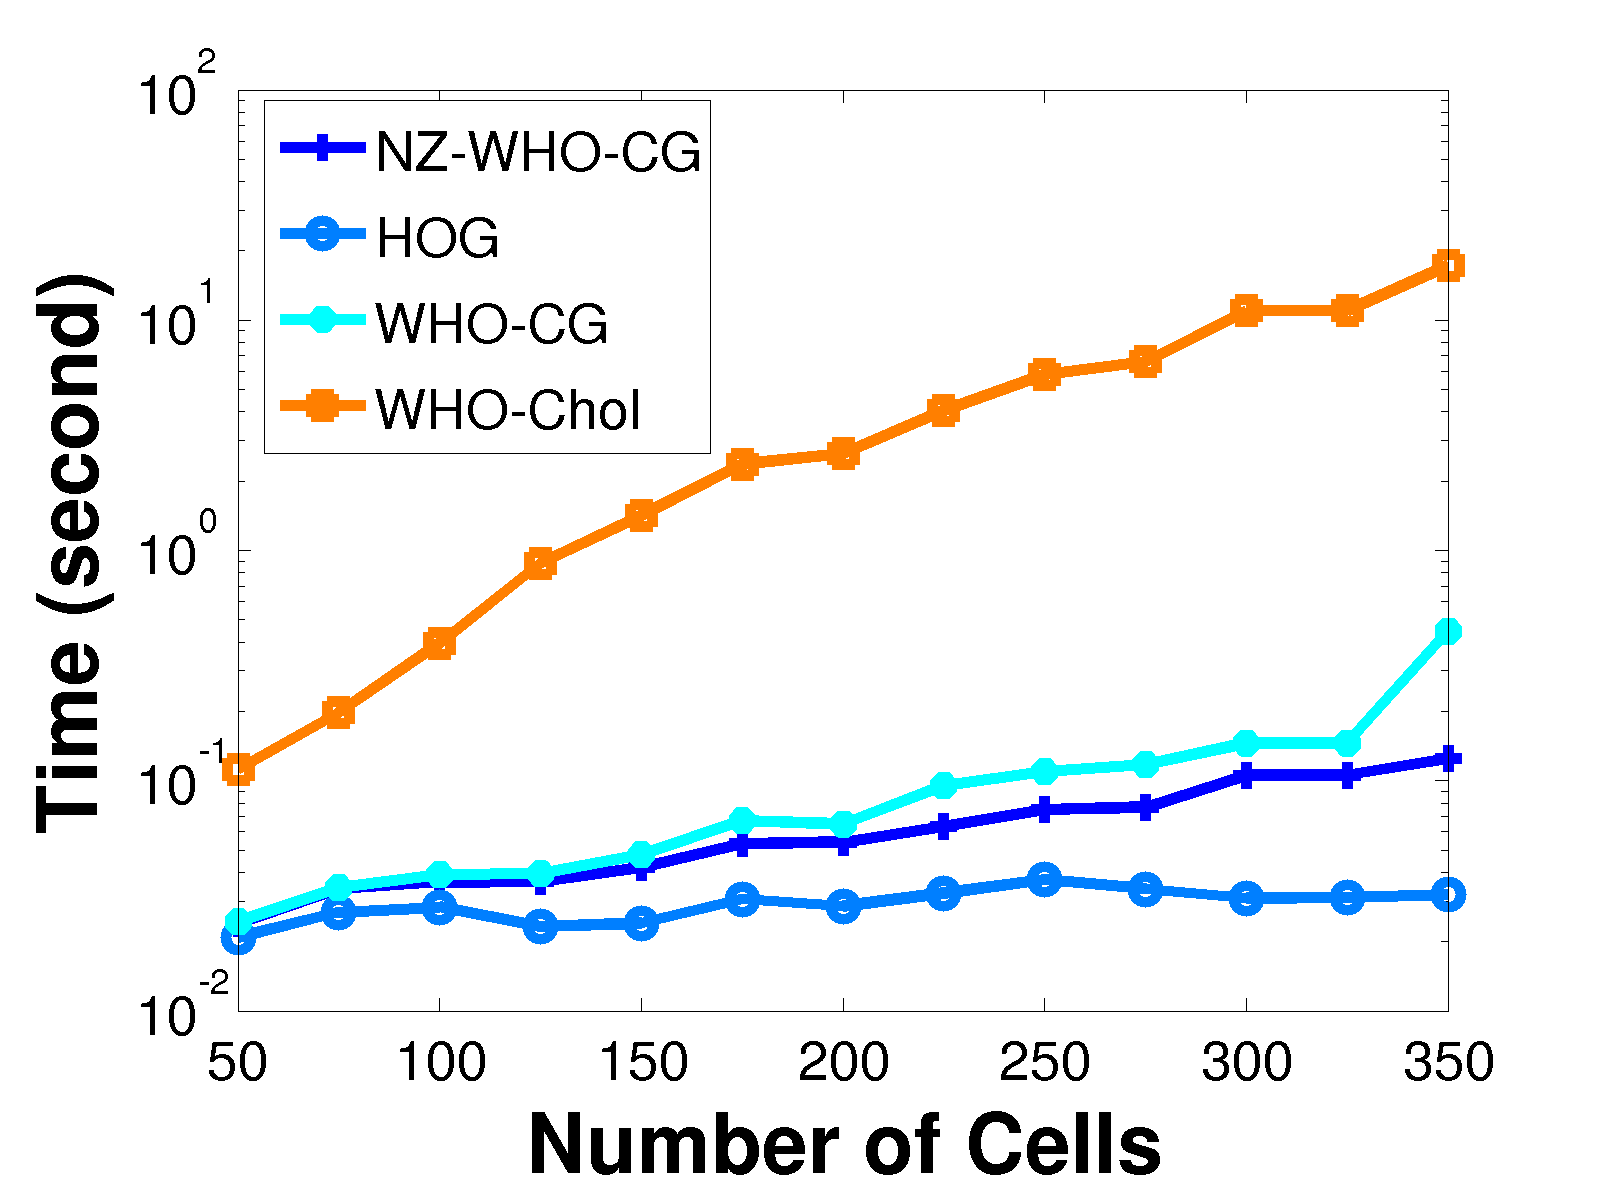
\includegraphics[width=0.5\linewidth]{whotime} & 
     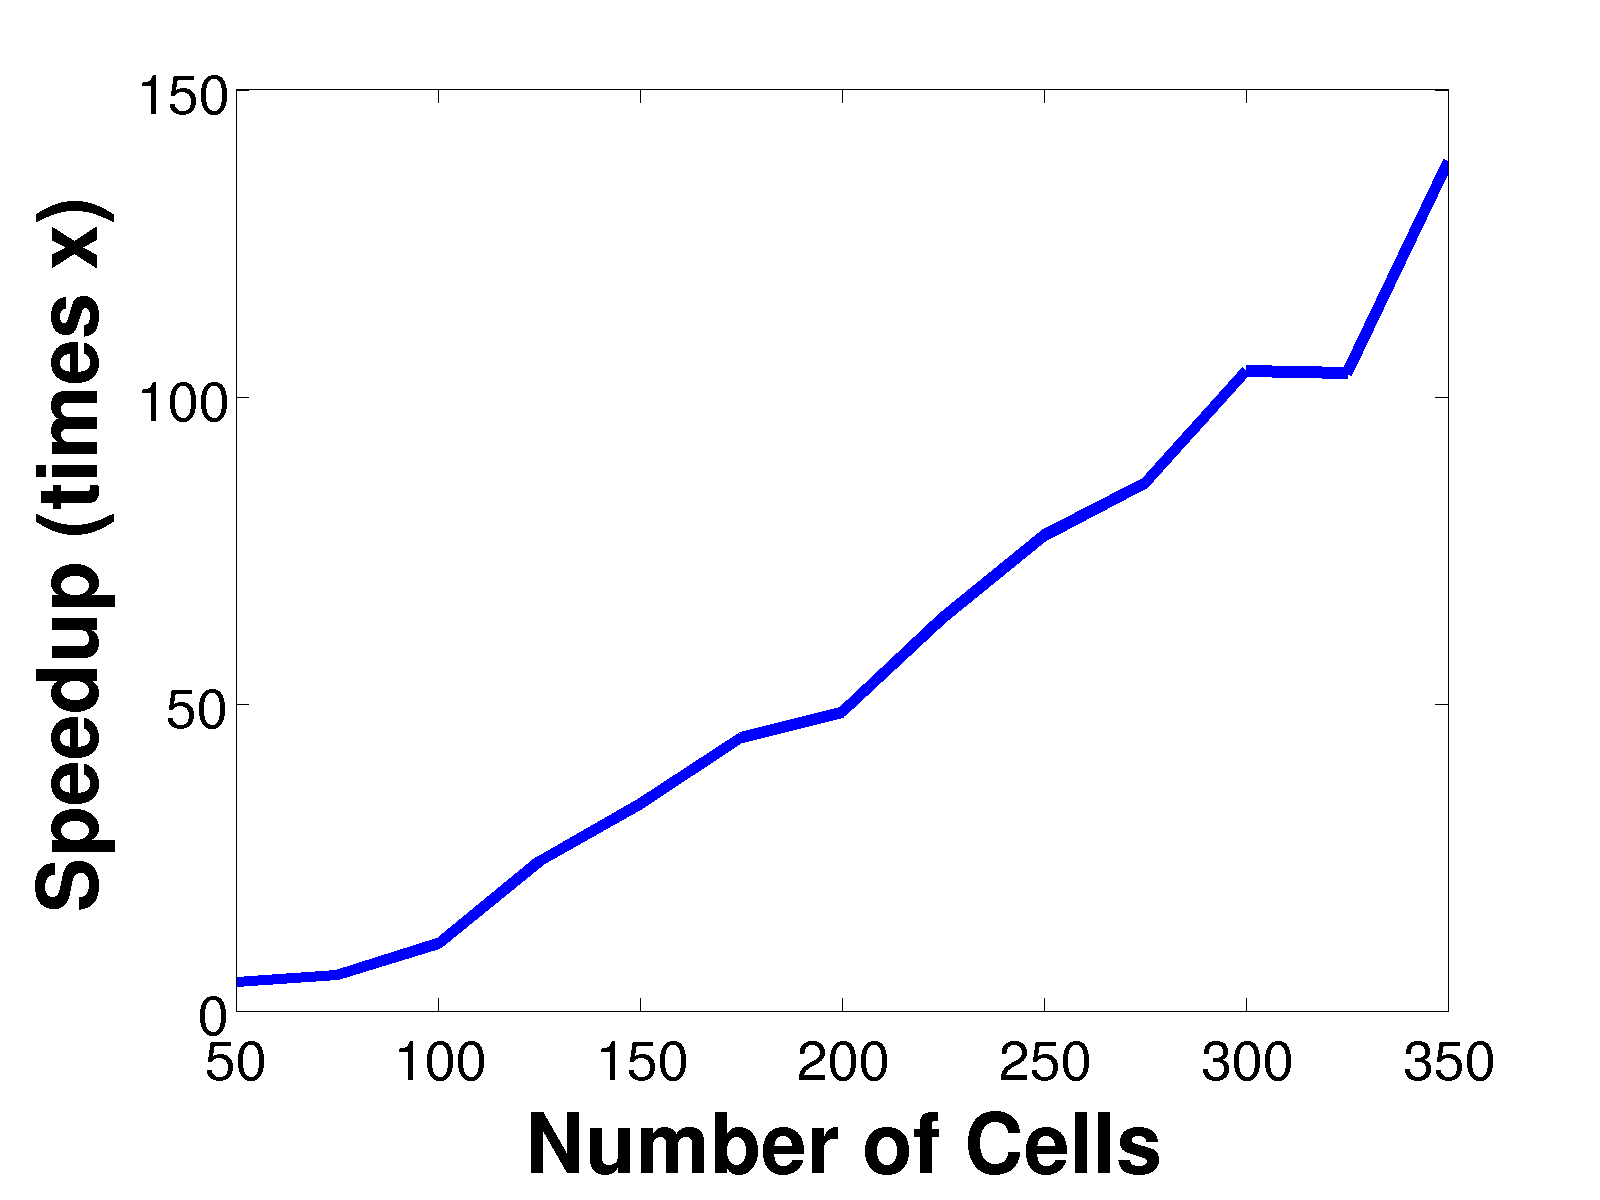
\includegraphics[width=0.5\linewidth]{speedup}\\
     (a) & (b) \\
 \end{tabular}
  \end{center}
  \caption{(a) Runtime analysis of whitening. HOG means feature
    extraction time, WHO-Chol uses ~\cite{Hariharan12} and
    WHO-CG uses iterative Conjugate Gradient. NZ-WHO-CG (Ours) uses only
    non-zero cells and Conjugate Gradient. (b) final speedup
    of NZ-WHO vs. WHO.}
  \label{fig:whotime}
\end{figure}
%
\begin{figure}[t]
  \centering
  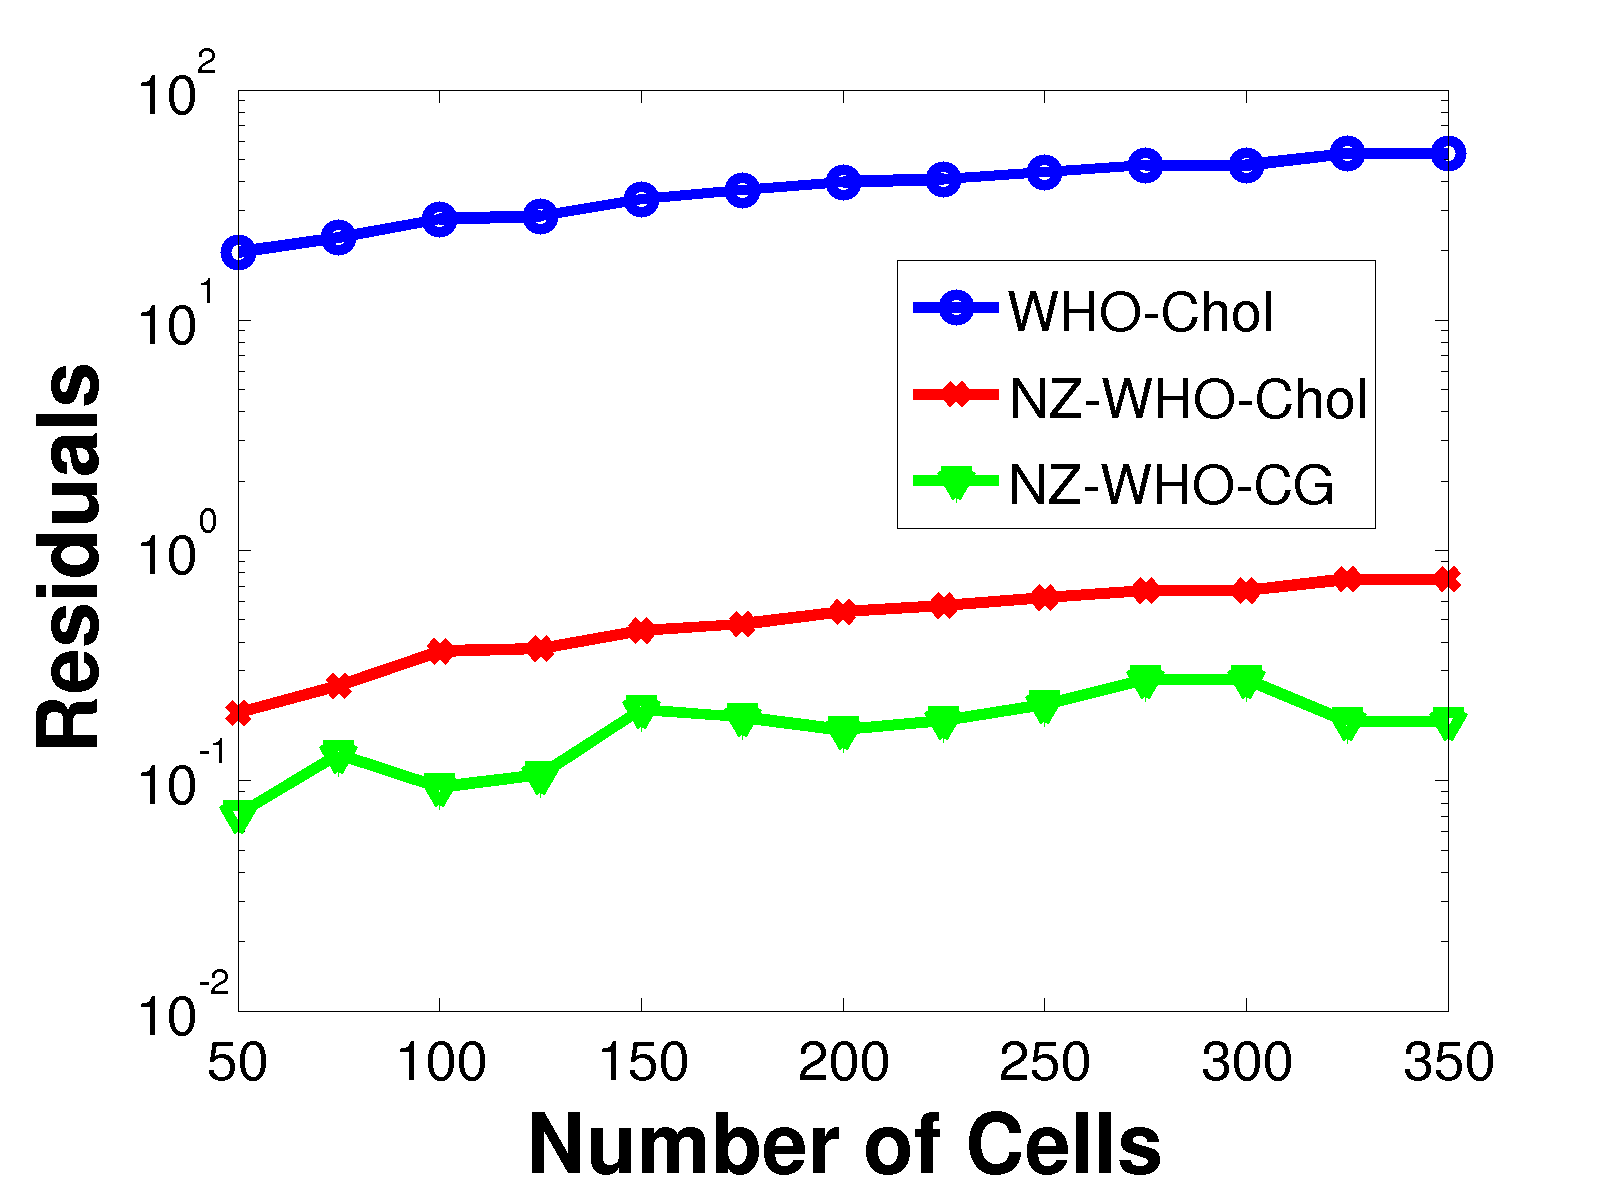
\includegraphics[width=0.5\linewidth]{residual}
  \caption{Residuals from different method}
  \label{fig:whoresidual}
\end{figure}


\subsection{High Resolution Templates and FFT based Convolution}
\label{sec:fft} 
We generate high resolution templates with more than 250 HOG cells to capture
details of an object to give accurate 2D-3D matching. These large templates
cause computational burden when computing convolution. Though good for
detecting accurate model and pose, convolution of high-resolution templates are
much slower since computation time scales linearly with the number of HOG
cells in the template. To overcome and speed up the convolution, we used FFT
based GPU convolution \cite{Podlozhnyuk} which scales. Briefly, for length $n$ signal and
length $m$ filter, naive convolution takes $O(nm)$ time whereas FFT-based
convolution takes $O\left( (n + m)\log (n+m) \right)$ time. For large
$m$ (high resolution templates), we can gain computational advantage.
